\chapter{結果}
\label{chap:results}
本章では、第3章で構築したデータセットおよび分析手法に基づき、松前町沿岸におけるマグロ延縄漁業の操業実態を可視化した結果について述べる。
まず、本研究で提案する「操業日誌データ」を用いた解析により、海域利用実態を明らかにする。次に、水揚げ記録をベースとした手法との比較を行い、手法の違いが可視化結果に与える影響を検証する。さらに、3カ年にわたる漁場形成の経年変化を示した上で、洋上風車建設予定海域との空間的な重複状況を評価する。最後に、洋上風車建設前の操業効率(CPUE・燃油効率)の分析結果を示す。

\section{利用頻度分布の可視化}
\subsection{操業日誌データに基づく操業実態の可視化}
2024年および2025年の操業日誌データに基づき、漁獲の有無に関わらず全ての操業における出港から入港までの航跡を反映させた利用頻度分布を、それぞれ図4.1aおよび図4.1bに示す。

\begin{figure}[htbp]
  \centering
  % 左側の図 (a)
  \begin{subfigure}[b]{0.48\textwidth}
    \centering
    \includegraphics[width=\textwidth]{images/2024m.png}
    \caption{2024年}
    \label{fig:2024m}
  \end{subfigure}
  \hfill
  % 右側の図 (b)
  \begin{subfigure}[b]{0.48\textwidth}
    \centering
    \includegraphics[width=\textwidth]{images/2025m.png}
    \caption{2025年}
    \label{fig:2025m}
  \end{subfigure}
  
  % 全体のキャプション
  \caption{操業日誌データに基づく利用頻度分布}
  \label{fig:log_frequency_dist}
\end{figure}

結果として、両年に共通して利用される海域と、年ごとに利用の有無が分かれる海域の双方が、明確に可視化された。
まず共通点として、両図ともに松前町沿岸から北西方向にかけて高頻度な漁場が形成されていることが分かる。この海域はマグロ延縄漁業の中核として恒常的に利用されていることが示された。
一方で、年ごとの分布形状には次のような差異が可視化されている。
2024年(図4.1a)では、操業が北西側の海域に強く偏在しているとともに、一部の航跡が南の津軽海峡方面へと直線的に伸びている様子が確認できる。
対して2025年(図4.1b)では、2024年には見られなかった南西側や、従来操業が少なかった海域へと、低い利用頻度の航跡が広く拡散している様子が捉えられている。


\subsection{水揚げ記録データに基づく操業実態の可視化}
次に、水揚げ記録とGNSS航跡データを照合し、漁獲実績のある日を抽出して作成した利用頻度分布を年順に、図\ref{fig:landing_dist}に示す。

\begin{figure}[H]
  \centering
  % 上段:2023年と2024年
  \begin{subfigure}[b]{0.48\textwidth}
    \centering
    \includegraphics[width=\textwidth]{images/2023g.png}
    \caption{2023年}
    \label{fig:2023g}
  \end{subfigure}
  \hfill
  \begin{subfigure}[b]{0.48\textwidth}
    \centering
    \includegraphics[width=\textwidth]{images/2024g.png}
    \caption{2024年}
    \label{fig:2024g}
  \end{subfigure}
  
  \vspace{1em} % 行間の調整

  % 下段:2025年(中央寄せ)
  \begin{subfigure}[b]{0.48\textwidth}
    \centering
    \includegraphics[width=\textwidth]{images/2025g.png}
    \caption{2025年}
    \label{fig:2025g}
  \end{subfigure}
  
  \caption{水揚げ記録に基づく利用頻度分布の経年変化}
  \label{fig:landing_dist}
\end{figure}

図\ref{fig:landing_dist}を参照すると、3カ年を通じて松前町沿岸北西部が中核的な漁場として機能している点は共通している。しかし、分布形状には年ごとに変化が見られる。
2023年(図\ref{fig:2023g})は、高頻度な海域が北西側に集中しており、利用頻度分布は3カ年の中で最も集中している。
2024年(図\ref{fig:2024g})では、依然として北西側が利用の中心となりつつも、南西側での利用が増えていることが確認できる。
2025年(図\ref{fig:2025g})では、高頻度域がより南西側へとシフトしている傾向が確認できる。特に2025年は、4.1.1項の操業日誌データに基づく利用頻度分布図(図\ref{fig:2025m})でも確認された通り、漁場が広範囲に分布している様子が本手法でも捉えられている。

\subsection{抽出手法による可視化結果の差異}
ここで、同一年(2024年または2025年)における「操業日誌ベース」と「水揚げ記録ベース」の結果を比較したものを、それぞれ図\ref{fig:compare_2024}、図\ref{fig:compare_2025}に示す。両年ともに、水揚げ記録ベースの利用頻度分布図の方が操業範囲が広く見えるものの、分布の見え方には大きな差は無かった。

\begin{figure}[H]
  \centering
  \begin{subfigure}[b]{0.48\textwidth}
    \centering
    \includegraphics[width=\textwidth]{images/2024m.png}
    \caption{操業日誌ベース}
    \label{fig:2024m_comp}
  \end{subfigure}
  \hfill
  \begin{subfigure}[b]{0.48\textwidth}
    \centering
    \includegraphics[width=\textwidth]{images/2024g.png}
    \caption{水揚げ記録ベース}
    \label{fig:2024g_comp}
  \end{subfigure}
  \caption{抽出手法による分布の比較(2024年)}
  \label{fig:compare_2024}
\end{figure}

\begin{figure}[H]
  \centering
  \begin{subfigure}[b]{0.48\textwidth}
    \centering
    \includegraphics[width=\textwidth]{images/2025m.png}
    \caption{操業日誌ベース}
    \label{fig:2025m_comp}
  \end{subfigure}
  \hfill
  \begin{subfigure}[b]{0.48\textwidth}
    \centering
    \includegraphics[width=\textwidth]{images/2025g.png}
    \caption{水揚げ記録ベース}
    \label{fig:2025g_comp}
  \end{subfigure}
  \caption{抽出手法による分布の比較(2025年)}
  \label{fig:compare_2025}
\end{figure}

以上の比較から、どちらの手法でも利用頻度分布の全体的な傾向や主要漁場の位置には大きな差異は見られなかった。すなわち、いずれの手法を用いても操業実態が可視化されており、主要な漁場の抽出には両手法とも有効であることが確認された。



\section{洋上風車建設予定海域との空間的重複}
4.1節で明らかになった操業実態と、洋上風力発電の導入が検討されている「促進区域」との空間的な重複状況を評価した結果を図\ref{fig:overlap}に示す。
ここでは、最も網羅性の高い「操業日誌ベース(2024年)」の利用頻度分布を背景に用い、その上に促進区域の輪郭線を黄色のラインで重ねて表示した。また、同漁協から提供された投縄開始地点も緑色の点でプロットしている。
南北方向に配列された地点群からは西側へ、東西方向に配列された地点群からは南側へと投縄が行われている。

\begin{figure}[H]
  \centering
   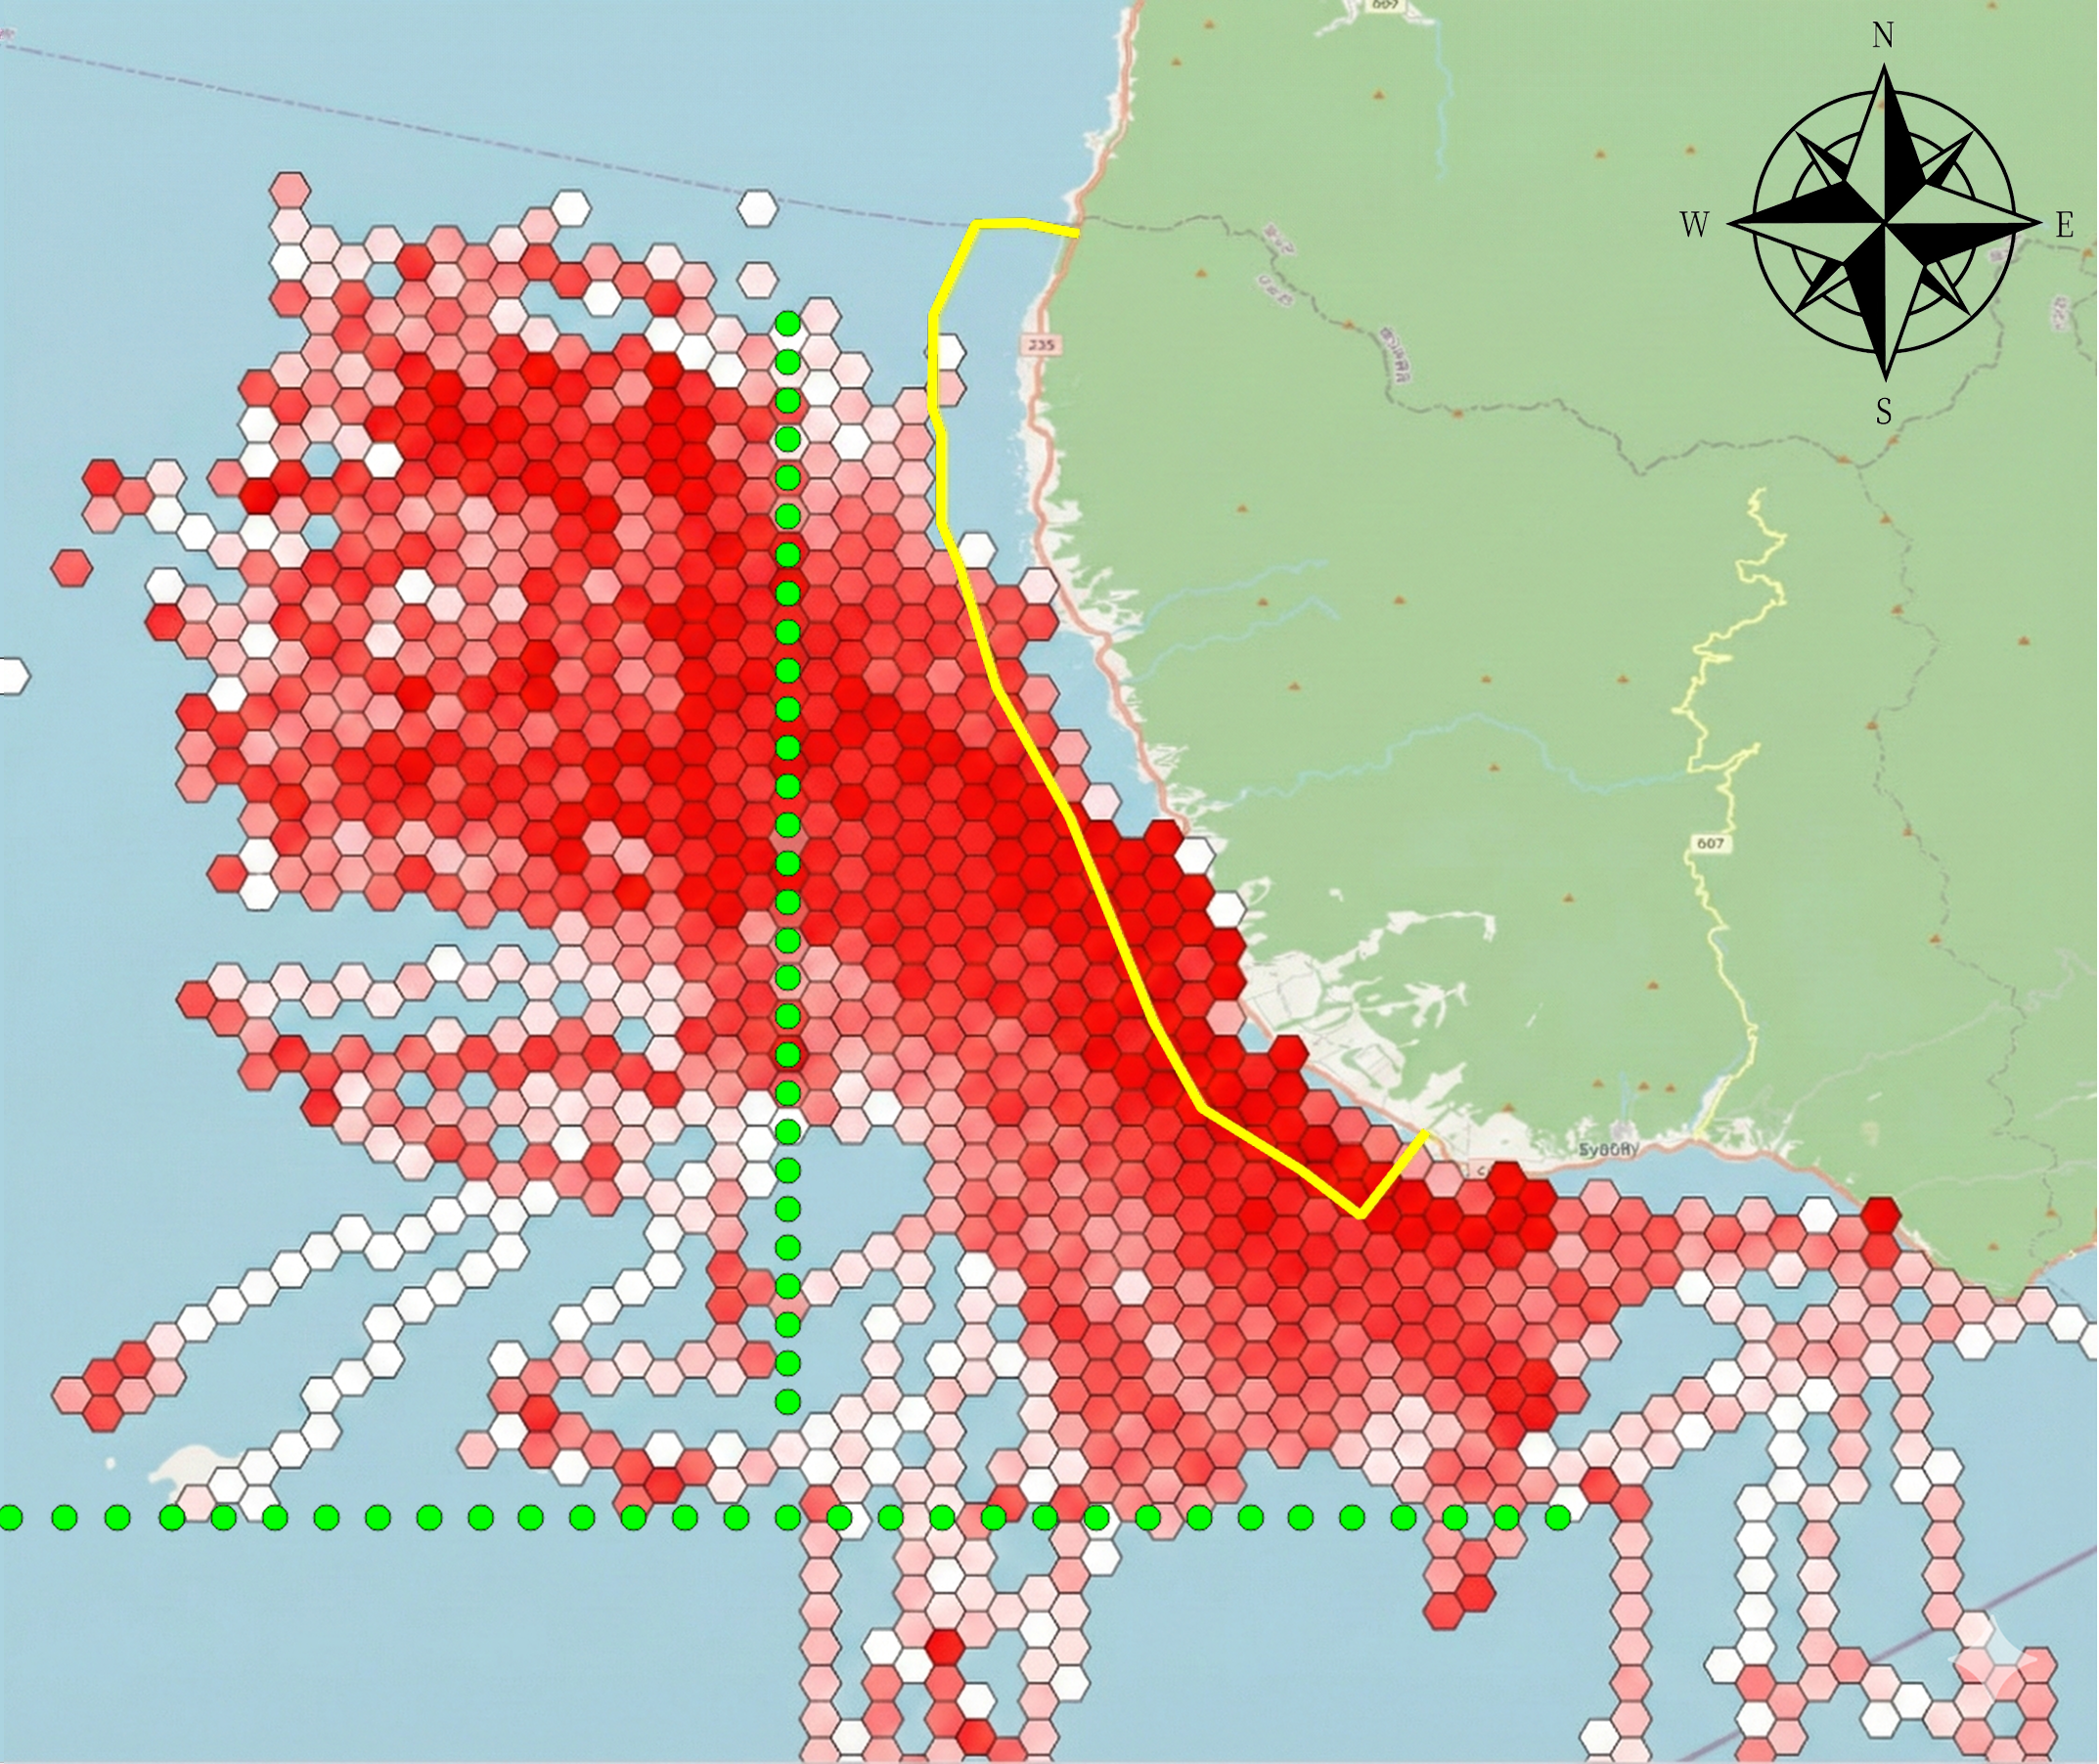
\includegraphics[width=12cm]{images/overlap.png}
  \caption{利用頻度と促進区域の空間的重複}
  \label{fig:overlap}
\end{figure}

図\ref{fig:overlap}を見ると、促進区域内側の南側には利用頻度が高いグリッドが複数存在しているが、緑色の点で示した投縄開始地点は促進区域から少なくとも2 nm 離れており、直接的な重複は確認されなかった。

\section{操業効率の現状評価}
本節では、4.1節で示された漁場の広範囲化、南西へのシフトの傾向が、コストに及ぼす影響を定量的に評価する。評価指標として、単位努力量あたりの漁獲量を示す CPUE および投入コストに対する生産性を示す燃油効率 ($E_o$)を用いて、2024年と2025年を比較した。

\subsection{CPUEの推移}
まず、漁獲量(kg)を総移動距離(nm)で除したCPUEの推移を評価する。1回の操業あたりの総移動距離を努力量とし、漁獲量との関係を図\ref{fig:cpue_scatter}に、漁期ごとの総漁獲量・総移動距離およびCPUEの比較を表\ref{tab:cpue_summary_updated}に示す。

\begin{figure}[H]
  \centering
   \includegraphics[width=12cm]{images/fig4_12_effort_vs_catch_scatter.png}
  \caption{1回の操業あたりの総移動距離と漁獲量の関係(2024年 vs 2025年)}
  \label{fig:cpue_scatter}
\end{figure}

\begin{table}[H]
  \centering
  \caption{漁期ごとのCPUEの比較}
  \label{tab:cpue_summary_updated}
  \begin{tabular}{lccc}
    \hline
    漁期 & 総漁獲量 (kg) & 総移動距離 (nm) & CPUE (kg/nm) \\
    \hline
    2024年 & 55,763 & 2,945.7 & 18.93 \\
    2025年 & 59,104 & 3,079.6 & 19.19 \\
    \hline
  \end{tabular}
  \begin{flushleft}
  \end{flushleft}
\end{table}

分析の結果、主要操業期間(7月〜11月)の総移動距離と総漁獲量に基づくと、2024年の年間平均CPUEは18.93 kg/nmであったのに対し、2025年は19.19 kg/nmとなり、結果として、CPUEは2024年と2025年で大きな違いは見られなかった。

\subsubsection{努力量と漁獲量の相関分析}
図\ref{fig:cpue_scatter}に示した散布図に基づき、移動距離が漁獲量にどの程度貢献したかを評価するため、両者の相関係数を算出した(表\ref{tab:correlation})。移動距離と漁獲量の関係性を評価するため、ピアソンの積率相関係数 ($R$) を算出し、無相関検定(両側t検定)を用いて統計的有意性を評価した。有意水準は 5\% ($p < 0.05$) とした。

\begin{table}[htbp]
  \centering
  \caption{移動距離と漁獲量の相関係数}
  \label{tab:correlation}
  \begin{tabular}{lcc}
    \hline
    漁期 & 総移動距離と漁獲量の相関係数 ($R$) & P値 \\
    \hline
    2024年 & 0.070 & 0.470 \\
    2025年 & 0.309 & $< 0.001$ \\
    \hline
  \end{tabular}
\end{table}

表\ref{tab:correlation}に示すように、2024年は相関係数が $R=0.070$ ($p=0.470$) であり、統計的に有意な相関は認められなかった。2025年は $R=0.309$ ($p < 0.001$) であり、弱い正の相関が確認された。

\subsection{燃油効率の推移}
投入された燃油に対する生産性を示す燃油効率($E_o$)の算出結果を表\ref{tab:fuel_efficiency}に示す。ここで、燃油使用量はGNSS航跡データと給油記録を統合し、給油間隔に基づく均等配分方式により各航跡ポイントに燃油使用量を配分して推定した値である。

\begin{table}[htbp]
  \centering
  \caption{漁期ごとの燃油効率(漁獲重量 / 推定燃油使用量)}
  \label{tab:fuel_efficiency}
  \begin{tabular}{lcccc}
    \hline
    漁期 & 総漁獲量 (kg) & 推定燃油使用量 (L) & 総量ベース $E_o$ (kg/L) & 月別平均 $\bar{E_o}$ (kg/L) \\
    \hline
    2023年 & 46,815 & 13,248 & 3.53 & 9.83 \\
    2024年 & 55,763 & 18,163 & 3.07 & 2.10 \\
    2025年 & 59,104 & 14,815 & 3.99 & 6.44 \\
    \hline
    全期間 & 161,681 & 46,226 & 3.50 & 6.36 \\
    \hline
  \end{tabular}
  \begin{flushleft}
    \small
    ※燃油使用量は、GNSS航跡データの各ポイントに給油間隔に基づき燃油使用量を配分して推定した値。
    ※給油記録が存在しない2隻については、全船平均の燃油消費率(0.106 L/ポイント)を適用。
  \end{flushleft}
\end{table}

表\ref{tab:fuel_efficiency}より、燃油効率は年度間で変動が見られる。2023年は9.83 kg/L、2024年は2.10 kg/L、2025年は6.44 kg/Lとなった。ただし、2023年については、VMSの導入が2023年6月中旬以降段階的に行われたため、漁期前半のデータが一部欠損しており、燃油使用量が過小評価されている可能性がある点に留意が必要である。具体的には、8月時点で稼働していたのは8隻のみであり、残りの21隻は9月以降に順次稼働を開始したため、2023年7〜8月の燃油効率は実態よりも高く算出されている可能性がある。

\subsection{月別燃油効率の変動特性分析}
年間を通じての効率の変動を把握するため、月別の燃油効率の推移を比較した(図\ref{fig:monthly_fuel_efficiency})。棒グラフは月別漁獲量(kg)を、折れ線グラフは燃油効率(kg/L)を示す。点線は期間平均燃油効率を表す。

\begin{figure}[H]
  \centering
  \includegraphics[width=14cm]{images/fig_monthly_fuel_efficiency_catch_fish.png}
  \caption{月別燃油効率と漁獲量の推移(2023年〜2025年)}
  \label{fig:monthly_fuel_efficiency}
\end{figure}

図\ref{fig:monthly_fuel_efficiency}を参照すると、2023年7〜8月は燃油効率が極端に高い値を示しているが、これはVMSの導入が2023年6月中旬以降に段階的に行われたためである。そのため、2023年7〜8月は漁獲量に対応する燃油使用量が十分に捕捉できておらず、燃油効率が過大評価されている。

そこで、VMSが概ね全船に導入された2023年9月以降のデータのみを抽出し、再度可視化を行った(図\ref{fig:monthly_fuel_efficiency_filtered})。

\begin{figure}[H]
  \centering
  \includegraphics[width=14cm]{images/fig_monthly_fuel_efficiency_catch_fish_filtered.png}
  \caption{月別燃油効率と漁獲量の推移(2023年9月〜2025年11月)}
  \label{fig:monthly_fuel_efficiency_filtered}
\end{figure}


図\ref{fig:monthly_fuel_efficiency_filtered}を参照すると、VMS導入初期を除外することで、より信頼性の高い燃油効率の季節変動が確認できた。2024年は7月に6.25 kg/L、8月に3.32 kg/Lと平均値の3.30 kg/L以上の効率を示したのち、9月以降は0.50 kg/L以下に低下した。2025年は7月に8.06 kg/L、8月に9.24 kg/Lを記録したのち、9月、10月に平均以下まで低下したものの、11月は12.62 kg/Lと高い値を示したことが特徴的である。

\subsection{月別CPUEの変動特性分析}
年間を通じての効率の変動を把握するため、月別のCPUEの推移を比較した(図\ref{fig:monthly_cpue})。

\begin{figure}[H]
  \centering
   \includegraphics[width=14cm]{images/fig_monthly_catch_cpue.png}
  \caption{月別CPUEと漁獲量の推移(2024年〜2025年)}
  \label{fig:monthly_cpue}
\end{figure}

図\ref{fig:monthly_cpue}を参照すると、2024年は7月が31.33 kg/nmでCPUEのピークとなり、1.75 kg/nmを記録した10月まで減少した後、11月にかけて0.80 kg/nmまで回復が見られた。2025年は8月が漁獲量が少ないものの、昨年の3倍以上である76.01 kg/nmのCPUEであった。各年ともに7月、8月が平均の22.27 kg/nm以上のCPUEを記録しており、漁期初期にCPUEが高い傾向が確認された。